\documentclass{article}
\usepackage{graphicx}
\usepackage[utf8x]{inputenc}
\usepackage[margin=1in]{geometry}
\usepackage{amsmath}
\usepackage{enumitem}
\usepackage{hyperref}
\usepackage{authblk}
\usepackage[british]{babel}
\usepackage{wrapfig}
\usepackage{layout}
\usepackage{flexisym}
\usepackage{listings}
\title{Transformations/Linear}


\title{Linear Algebra/Intro to Transformations}

\author{Ajith Kemisetti}
\affil{Computer Vision Club}
\date{January 2017}

\begin{document}

\maketitle

\section{Introduction}

Linear algebra forms the mathematical basis for Computer Vision, since images are typically represented as matrices of pixel intensities. This lecture will explain the role that linear algebra plays in Computer Vision as well as linear transformations and how they work with respect to the matrix representation of the image. Rather than explain linear algebra and transformations as separate topics, this lecture will only talk about them together in context of Computer Vision, since understanding them is an important prerequisite to other topics.

\section{2D Transformations}

\begin{wrapfigure}{r}{0.75\textwidth}
  \begin{center}
    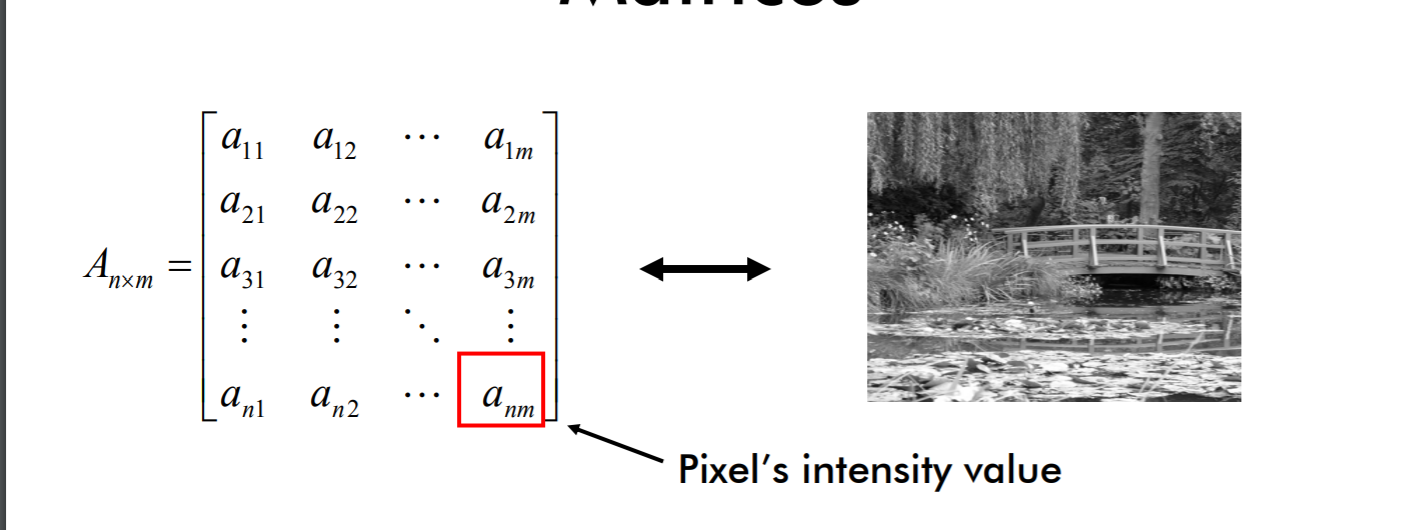
\includegraphics[width=0.8\textwidth]{matrixIntensity.png}
  \end{center}
  \caption{Matrix Representation of Image}
\end{wrapfigure}
The matrix on the right is a very straightforward depiction of matrices to represent images. In order to perform manipulations on the images, usually the "intensity" matrix will be the go-to . The first type of transformations include 2D Geometric Transformations (Rotation, Translation, and Scaling). There are functions in OpenCV that can perform these transformations on images pretty easily for you and understanding what these functions are doing shouldn't be a challenge. For that reason, the actual code for this will be left as an exercise and focus will be put on a mathematical understanding on what is going on. But there are more difficult transformations for which seeing the code for is essential in order to understand them. Examples for today will include Affine Transformations, Perspective Distortion Removal, and Direct Linear Transformation. 
\section{Homogenous Coordinates}

The fundamental coordinate system of computer vision is the system of homogeneous coordinates. Homogeneous coordinates can be thought of projecting all the points on the image to an additional dimension. Mathematically they are actually very easy to represent. While you may be able to do transformations such as translation, rotation, and scaling with 2D matrices, a homogeneous coordinate system is absolutely necessary if we wanted to do something like transforming an image of a building to show a bird's eye view \textbf{ given an image of the building viewed from the front}. 

Going back and forth between Cartesian and homogeneous is fairly straightforward: 
\begin{center}
\begin{math}(x,y) \rightarrow (x*z,y*z,z),  z \ne 0 \end{math} \\
\end{center}
All that needs to be done is for x and y to be multiplied by some non zero scalar \begin{math}z\end{math}. Can be applied for fourth dimensions as well. Conventionally the scalar is chosen to be 1.
\[
\begin{bmatrix}
    x\\
    y
\end{bmatrix}
\rightarrow
\begin{bmatrix}
    x\\
    y\\
    z
\end{bmatrix}
\]
When doing transformations in general (and this is something that is true for the general field of linear algebra as well) transformation matrices are used to encompass all the information regarding the transformation. This information can include how large the new vector will be as well as where the vector is going to go. \\
If we call the transformation matrix \begin{math} T \end{math}
then whatever happens to \begin{math} (x,y,z) \end{math} can be expressed through matrix multiplication as follows: \\
\[
T
*
\begin{bmatrix}
    x\\
    y\\
    1
\end{bmatrix}
=
\begin{bmatrix}
    $x\textprime$\\
    $y\textprime$\\
    1
\end{bmatrix}
\]
It would be too cumbersome to talk about the transformation matrices for translation, rotation, and scaling individually. Thankfully, all of these operations can be done at once by simply stating: \\
Let \begin{math}P\end{math} be the original matrix \\
\[
\begin{bmatrix}
    1 & 0 & tx \\
    0 & 1 & tx \\
    0 & 0 & 1\\
\end{bmatrix}
*
\begin{bmatrix}
    \cos{\theta} & -\sin{\theta} & 0\\
    \sin{\theta} & \cos{\theta} & 0\\
    0 & 0 & 1\\
\end{bmatrix}
*
\begin{bmatrix}
    sx & 0 & 0 \\
    0 & sy & 0 \\
    0 & 0 & 1\\
\end{bmatrix}
*
\begin{bmatrix}
    x\\
    y\\
    1
\end{bmatrix}
=
P\textprime
\]

Where \begin{math}\theta\end{math} is degrees of rotation, 
tx and ty are how far right/left and how far up/down the figure should move, respectively, and sx and sy represent scaling factors for x and y, respectively. 
\section{Affine and Perspective Transformations}

Properties of an Affine Transformation: \\
\begin{itemize}
  \item Straight Lines, points, and planes are preserved \begin{math}A[r,\theta]\end{math} in the parameter space
  \item Lines parallel in the original image will remain parallel
  \item Angles between lines or distances between points are not preserved
  \item Ratios of distances between points lying on a straight line aren't preserved
\end{itemize}

Transformations like Affine Transformations are the reason why homogeneous coordinates are needed in computer vision. An extra dimension is necessary in order to warp the image to show different viewpoints of it. \\
As previously discussed, all transformations to the intensity matrix of the image are determined by a transformation matrix. An intuitive grasp of what the transformation matrix would look like is far more difficult with transformations like the ones on the right. Qualitatively, on the other hand,  imagining the projection of the image onto a 3D homogeneous coordinate plane being rotated to visualize the affine transformation is quite simple. OpenCV will use 3 sets of before-after points to approximate what this matrix will look like and perform use that matrix on the rest of the image. \\
\begin{lstlisting}
img = cv2.imread('myCar.png')
rows,cols,ch = img.shape
pts1 = np.float32([[50,50],[200,50],[50,200]])
pts2 = np.float32([[10,120],[200,80],[100,290]])
M = cv2.getAffineTransform(pts1,pts2)
dst = cv2.warpAffine(img,M,(cols,rows))
plt.subplot(121)
plt.imshow(img)
plt.title('Before Affine')
plt.subplot(122)
plt.imshow(dst)
plt.title('AFter Affine')
plt.show()
\end{lstlisting}
As long as you have a rough idea on where you want 3 points in your image to be located after the transformation, OpenCV will take care of the rest of the image. Perspective Transform is basically the same thing except for the fact that 4 points are required. This would also make for a very quick but useful exercise (the OpenCV python API makes it very clear how to do this).

\begin{wrapfigure}{r}{0.4\textwidth}
  \begin{center}
    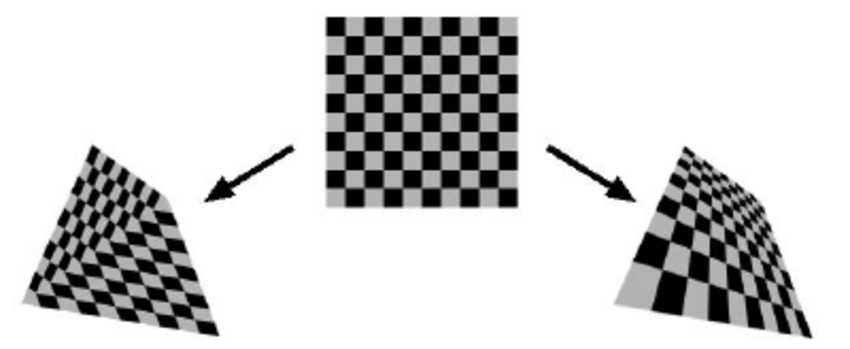
\includegraphics[width=0.4\textwidth]{affineChess.png}
  \end{center}
  \caption{Examples of an Affine Transformation}
\end{wrapfigure}

\section{Homography}
Images taken from different perspective of the same object will have corresponding points. For example, if pictures were to be taken of a pencil but each from a different perspective, the tip of the pencil would be at a different place in each image, even though the images are of the same object. While seemingly intuitive, computing a matrix to model this transformation is difficult, to the point where the setup will be shown but the full solution would take longer than what time permits. For that reason, in section 6 a link will be provided for a full solution. The algorithm is called Direct Linear Transformation (DLT) \\ \\ 
\[
H _{homography matrix} =
\begin{bmatrix}
    h_{11}       & h_{12} & h_{13} \\
    h_{21}       & h_{22} & h_{23} \\
    h_{31}       & h_{32} & h_{33} \\
\end{bmatrix} 

\\ H
*
\begin{bmatrix}
    x_{2}\\
    y_{2}\\
    1
\end{bmatrix}
=
\begin{bmatrix}
    x_{1}\\
    y_{1}\\
    1
\end{bmatrix} \\
The mapping will operate on the new points (x2,y2) and
associate them with (x1,y1) for every point in image. As previously stated, the solution will be in the references section. The code is as follows:
\]
\begin{lstlisting}
import cv2
import numpy as np
im_src = cv2.imread('book1.jpg')
# Four corners of the book in source image
pts_src = np.array([[141, 131], [480, 159], [493, 630],[64, 601]])
pts_dst = np.array([[0, 0],[299, 0],[299, 399],[0, 399]])
h, status = cv2.findHomography(pts_src, pts_dst,cv2.RANSAC,5.0)
# Warp source image to destination based on homography
im_out = cv2.warpPerspective(im_src, h, (399,299))
cv2.imshow("Source Image", im_src)
cv2.imshow("Corrected Source Image", im_out)
cv2.waitKey(0)
\end{lstlisting}
OpenCV will roughly approximate a homography matrix given an image
modeling the warping that took place and can even apply that same warping to a new image. While warping images isn't useful, what is useful about having a matrix that models imperfections in the image is the ability to make a perspective correction based on that. This is what the above code does.

\section{Exercises + Extra Links}
The following exercises will get progressively more difficult and are not mandatory. But doing them will ensure an understanding on how to effectively apply the topics covered in code, which is the most important skill of all.
\begin{enumerate}
  \item Write a program to take any image and move it 50 pixels right and 100 pixels down and then rotate it 90 degrees.
  \item Write a program to zoom in on an image . User input isn't necessary. Just use your own discretion to make sure that it looks like a closeup of some aspect of the image is being shown. 
  \item Write a program that uses feature matching and homography to draw lines between a picture of 1 bird and a picture of a flock of birds. You may use OpenCV's APIs and if you search for feature matching then it should become clear to you what is being asked.
\end{enumerate}
Link (for the full homography derivation):
http://web.eecs.umich.edu/~silvio/teaching/lectures/lecture2.pdf
Slide 47 OR Just google "linear algebra computer vision" and the second link should be the powerpoint. Skip to slide 47.

\end{document}